\section{Evaluation}
\label{sec:eval}
We first present the experimental setup, followed by results on cue discovery, 
model probing, and analysis. 
The entire framework is implemented in an online demo. 
%~\footnote{\url{https://github.com/flora336/icq} 
%\KZ{Make sure this demo is live all the time, and
%is the code and data also located here?}}.

\subsection{Setup} 
We evaluate this framework on 10 popular NLR datasets in ~\tabref{tab:datasets} and
4 well-known models, namely FASTText (FT)~\cite{joulin2017bag}, 
ESIM (ES)~\cite{chen2016enhanced}, BERT (BT)~\cite{devlin2018bert} and RoBERTA (RB)~\cite{liu2019roberta}
on these datasets. All these datasets except for 
SWAG~\cite{zellers2018swag} and RECLOR~\cite{yu2020reclor} are collected
through crowdsourcing. SWAG is generated from an LSTM-based language model.
Specifications of the datasets are listed in \tabref{tab:datasets}.

\begin{table}[th]
\centering
\scriptsize
%\begin{tabular}{l|c|c|c|c}
\begin{tabular}{p{0.06\textwidth}
>{\centering}p{0.06\textwidth}
>{\centering}p{0.06\textwidth}
>{\centering}p{0.06\textwidth}
c}
%\begin{tabular}{p{1.5cm}>{\centering}p{1cm}>{\centering}p{1cm}>{\centering}p{1cm}>{\centering}p{1cm}p{1cm}}
\toprule
Dataset & Type & Data Size & Train/Test & Human Acc\\ \cmidrule{4-4} \cmidrule{5-5}
 	&	&	& Ratio	& (\%) \\ 
\midrule
SNLI     &CLS   &  570K     & 56:1               &80.0\\
QNLI     &CLS    & 11k         &  19:1           &80.0\\
MNLI     &CLS     & 413k       &  40:1             &80.0\\
ROC & MCQ & 3.9k         & 1:1            &100.0  \\
COPA     &MCQ    & 1k           &  1:1         & 100.0     \\
SWAG     &MCQ   & 113k       &  4:1             & 88.0\\
RACE     & MCQ   & 100k      &  18:1              &94.5\\
RECLOR   &MCQ    &  6k          &  9:1           &63.0\\
%CQA      &MCQ   & 12k        &  9:1                &88.9\\
ARCT     &MCQ    & 2k         & 3:1                &79.8\\
ARCT\_adv& MCQ & 4k         & 3:1                 & -\\
\bottomrule
\end{tabular}
\caption{10 Datasets. Data size refers to the number of questions
in each dataset. CLS=Classification. MCQ=Multiple Choice Questions. 
By our definition, $k$-way MCQs will be split into $k$ instances 
in preprocessing.}\label{tab:datasets} 
\end{table}

%\KZ{Add some new datasets including aNLI.} 
These datasets can mainly be classified into two types of tasks. 
SNLI, QNLI, and MNLI~\cite{WilliamsNB18} are classification tasks, while 
ROC, COPA~\cite{roemmele2011choice}, SWAG, 
RACE~\cite{lai2017race}, 
RECLOR, %CQA~\cite{talmor2019commonsenseqa}, 
ARCT~\cite{habernal2017argument} and ARCT\_adv~\cite{schuster2019towards} are
multiple-choice reasoning tasks. 
Features appearing a minimum of five times in training or testing sets are considered cues.


\subsection{Cues in Datasets} 

In this section, we showcase the cues identified in each dataset using 
the cueness metric, as described in \secref{sec:approach}. 

We first filter the training and test data for each dataset using all the features defined in this paper. The left half of \tabref{tab:bias} displays the top 5 cues discovered for each of the 10 datasets, along with their cueness scores. ARCT\_adv, an adversarial dataset, is intentionally well-balanced. Consequently, we only found one cue, OVERLAP, with a very low cueness score. This is unsurprising since OVERLAP is the only ``second-order'' feature in our list of linguistic features that considers tokens in both the premise and hypothesis, and likely evaded data manipulation by the creator.

Mostly, the top 5 cues discovered are word features. However, besides OVERLAP, we also see NEGATION and TYPO appearing in the lists. In fact, SENTIMENT and NER features would have emerged if we expanded the list to the top 10. Interestingly, several features previously reported as biased by other works, such as ``not'' and NEGATION in ARCT, ``no'' in MNLI and SNLI, and ``like'' in ROC, are also found. Particularly in MNLI, all five discovered cues are related to negatively toned words, suggesting significant human artifacts in this dataset that can lead to model fragility.

Additionally, we observe that some word cues are indicative of certain syntactic, semantic, or sentiment patterns in the questions. For example, ``because'' in SNLI implies a cause-effect structure; ``like'' in ROC indicates positive sentiment; ``probably'' and ``may'' in RACE suggest uncertainty, and so on. These features can serve as clues for revising datasets.

%\begin{table}[p] 
\begin{table*}[ht]
\centering
\scriptsize
%\begin{tabular}{c|c|c|c|c|c|c} \hline
\begin{tabular}{p{0.08\textwidth}
>{\centering}p{0.08\textwidth}
>{\centering}p{0.08\textwidth}
>{\centering}p{0.08\textwidth}
>{\centering}p{0.08\textwidth}
>{\centering}p{0.08\textwidth}
c}
\toprule
Dataset & Top Cues & Cueness & FT  & ES & BT & RB\\ 
	&	& \%	& ($\Delta$)& ($\Delta$)& ($\Delta$)& ($\Delta$) \\ \hline
\multirow{5}{*}{SNLI} 
& ``sleeping'' & 13.95 & 30.3 &6.81 & 5.34& 4.87 \\                                                                    
& ``no'' & 13.33 & 18.09 &3.32 & 2.05& 2.6 \\
& ``because'' & 9.24 & 18.89 &4.88 & 5.61& 4.31 \\
& ``friend'' & 8.82 & 22.96 &6.66 & 3.51& 3.05 \\
& ``movie'' & 7.73 & 16.64 &0.06 & 9.47& -0.19 \\
	   \midrule 
\multirow{5}{*}{QNLI} 
& ``dioxide'' & 4.52 & 9.78 &-0.06 & 4.97& 10.56 \\                                                                    
& ``denver'' & 4.26 & 13.59 &7.14 & 2.23& 3.11 \\
& ``kilometre'' & 4.24 & 4.85 &6.43 & 4.67& 2.55 \\
& ``mile'' & 3.95 & 7.16 &15.64 & -1.65& -6.65 \\
& ``newcastle'' & 3.8 & 3.44 &12.0 & 0.89& -1.23 \\
	   \midrule 
\multirow{5}{*}{MNLI} 
& ``never'' & 10.4 & 29.15 &26.41 & 9.86& 10.6 \\                                                                      
& ``no'' & 8.98 & 19.49 &20.17 & 1.2& 3.32 \\
& ``nothing'' & 8.98 & 25.5 &26.84 & 5.11& 4.32 \\
& ``any'' & 6.79 & 20.4 &19.39 & 7.76& 3.74 \\
& ``anything'' & 5.73 & 18.43 &15.74 & 3.31& 1.14 \\
	   
	   \midrule 
\multirow{5}{*}{ROC} 
& ``threw'' & 12.99 & 1.28 &4.69 & 10.88& 0.97 \\                                                                      
& ``now'' & 8.68 & -10.01 &14.51 & 1.75& 5.69 \\
& ``found'' & 8.16 & -2.31 &4.45 & 5.12& -3.13 \\
& ``won'' & 7.71 & 2.43 &0.74 & 1.05& 5.51 \\
& ``like'' & 7.3 & 4.77 &10.06 & 8.81& 1.67 \\
	   \midrule 
\multirow{5}{*}{COPA} 
& ``went'' & 3.61 & -10.83 &6.46 & 7.92& 1.04 \\                                                                       
& ``got'' & 2.74 & 5.45 &-9.89 & -12.52& -10.3 \\
& ``for'' & 2.14 & 10.11 &-1.89 & 9.05& 11.58 \\
& ``with'' & 1.38 & -15.64 &-6.98 & 3.3& 13.82 \\
& TYPO & 0.84 & -12.46 &-2.33 & 3.8& -8.22 \\
	   \midrule 
\multirow{5}{*}{SWAG}
& ``football'' & 7.38 & 6.13 &8.55 & 1.2& 1.55 \\
& ``anxious'' & 6.65 & 7.55 &-4.67 & -6.66& -1.67 \\
& ``concerned'' & 6.19 & 12.6 &4.58 & 8.27& -5.66 \\
& ``skull'' & 5.73 & -2.77 &0.49 & 8.43& 3.49 \\
& ``cop'' & 5.01 & 2.79 &5.3 & -0.92& -0.04 \\
	   \midrule 

\multirow{5}{*}{RACE} 
& ``above'' & 13.74 & 8.73 &-8.43 & -0.22& -1.92 \\                                                                    
& ``b'' & 12.84 & 16.97 &-4.8 & 3.52& -3.45 \\
& ``c'' & 11.83 & 15.69 &-6.94 & 8.6& -7.6 \\
& ``probably'' & 6.77 & 9.91 &-0.06 & -3.8& 2.86 \\
& ``may'' & 4.2 & 7.75 &-3.45 & -6.67& -1.8 \\
	   
	   \midrule 
\multirow{5}{*}{RECLOR} 
& ``over'' & 2.07 & 1.76 &-2.94 & -1.35& -4.12 \\                                                                      
& ``result'' & 1.97 & -3.29 &-2.69 & -1.78& -3.7 \\
& ``explanation'' & 1.81 & -6.33 &-1.73 & -2.76& -7.24 \\
& ``proportion'' & 1.68 & -5.64 &-4.69 & 2.37& -2.16 \\
& ``produce'' & 1.4 & 4.54 &-2.98 & -14.36& -3.7 \\
	   \midrule 
\multirow{5}{*}{ARCT} 
& ``not'' & 3.74 & -2.54 &7.45 & -0.97& -11.96 \\                                                                      
& NEGATION & 2.85 & 3.49 &10.04 & 6.28& -8.23 \\
& ``n't'' & 2.52 & 10.3 &5.89 & 9.49& 4.84 \\
& ``always'' & 2.25 & -4.66 &38.21 & -4.35& -8.26 \\
& ``doe'' & 2.06 & -0.73 &-3.69 & -1.15& -7.22 \\
	   \midrule 
ARCT\_adv& OVERLAP & 1.96e-10 & 1.65 &-0.25 & 2.73& 0.57 \\ \midrule
\multicolumn{3}{c|}{$\sum(|.|)$ (Model weakness)} 	& 469.8 & 361.4 & 227.7 & 216.2 \\
\bottomrule 
\end{tabular}
\caption{Datasets, their top 5 cues and 4 models biases $\Delta$ on them.}
\label{tab:bias}
\end{table*}


\subsection{Biases in Models}
To investigate whether a model is affected by a specific cue or feature in a dataset, we train four models on their original training sets and evaluate them using accuracy and distribution tests.

\textbf{Accuracy Test:} The results are presented in \tabref{tab:bias}. 
As mentioned in~\secref{sec:accuracytest}, a positive or negative $\Delta$ 
value indicates the direction of a model's performance change when comparing 
its accuracy on data subsets with and without specific features. 
The absolute value of $\Delta$ reflects the degree to which 
the model's performance is influenced by these features, 
with larger values suggesting stronger reliance or sensitivity and smaller values indicating a more robust model. 

The bottom of \tabref{tab:bias} shows that, 
across all 10 datasets, the sum of the absolute 
values of $\Delta$ follows the order: RoBERTA $<$ BERT $<$ ESIM $<$ FastText. This is consistent with earlier hypothesis-only tests and the community's common perception of these popular models. However, examining individual datasets and features reveals a more nuanced situation. For instance, FastText tends to pick up individual word cues rather than semantic cues, while more complex models such as BERT and RoBERTA appear more sensitive to structural features like NEGATION and SENTIMENT, which are actually classes of words. This is well explained by FastText's design, which focuses more on modeling words than syntactic or semantic structures.

Interestingly, FastText exhibits a strong negative correlation with TYPO. We speculate that FastText might have been trained with a more orthodox vocabulary, making it less tolerant of typos in the text.

\begin{figure}[th]
\centering
\begin{minipage}[b]{0.45\linewidth}
\centering
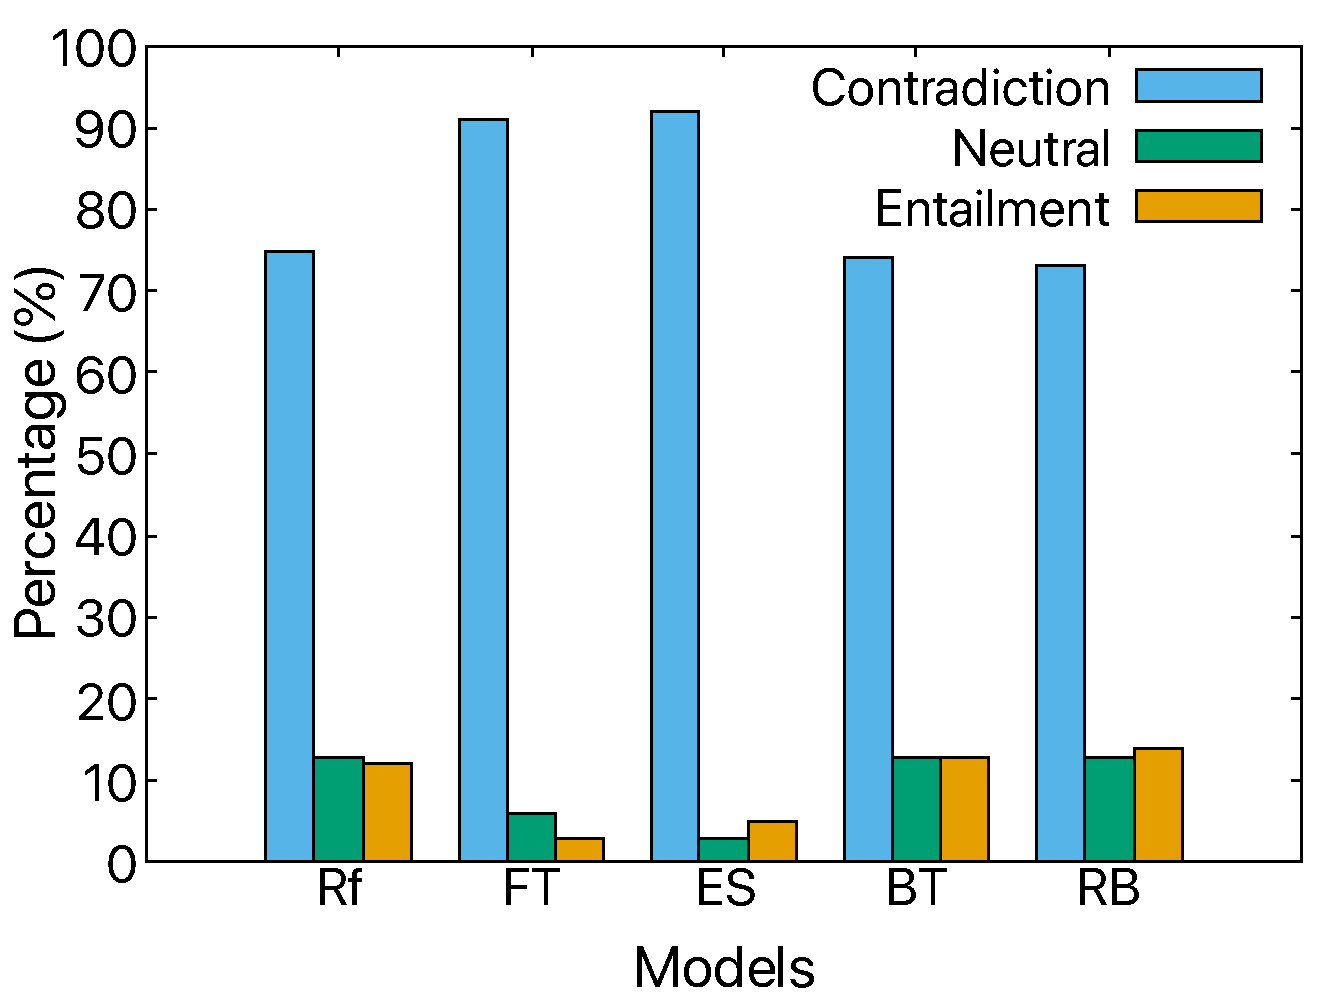
\includegraphics[width=\columnwidth]{picture/no-mnli.pdf}
\caption*{Cue ``no'' in MNLI} 
\label{fig:cue_no} 
\end{minipage}
\hspace{0.5cm} 
\begin{minipage}[b]{0.45\linewidth} 
\centering 
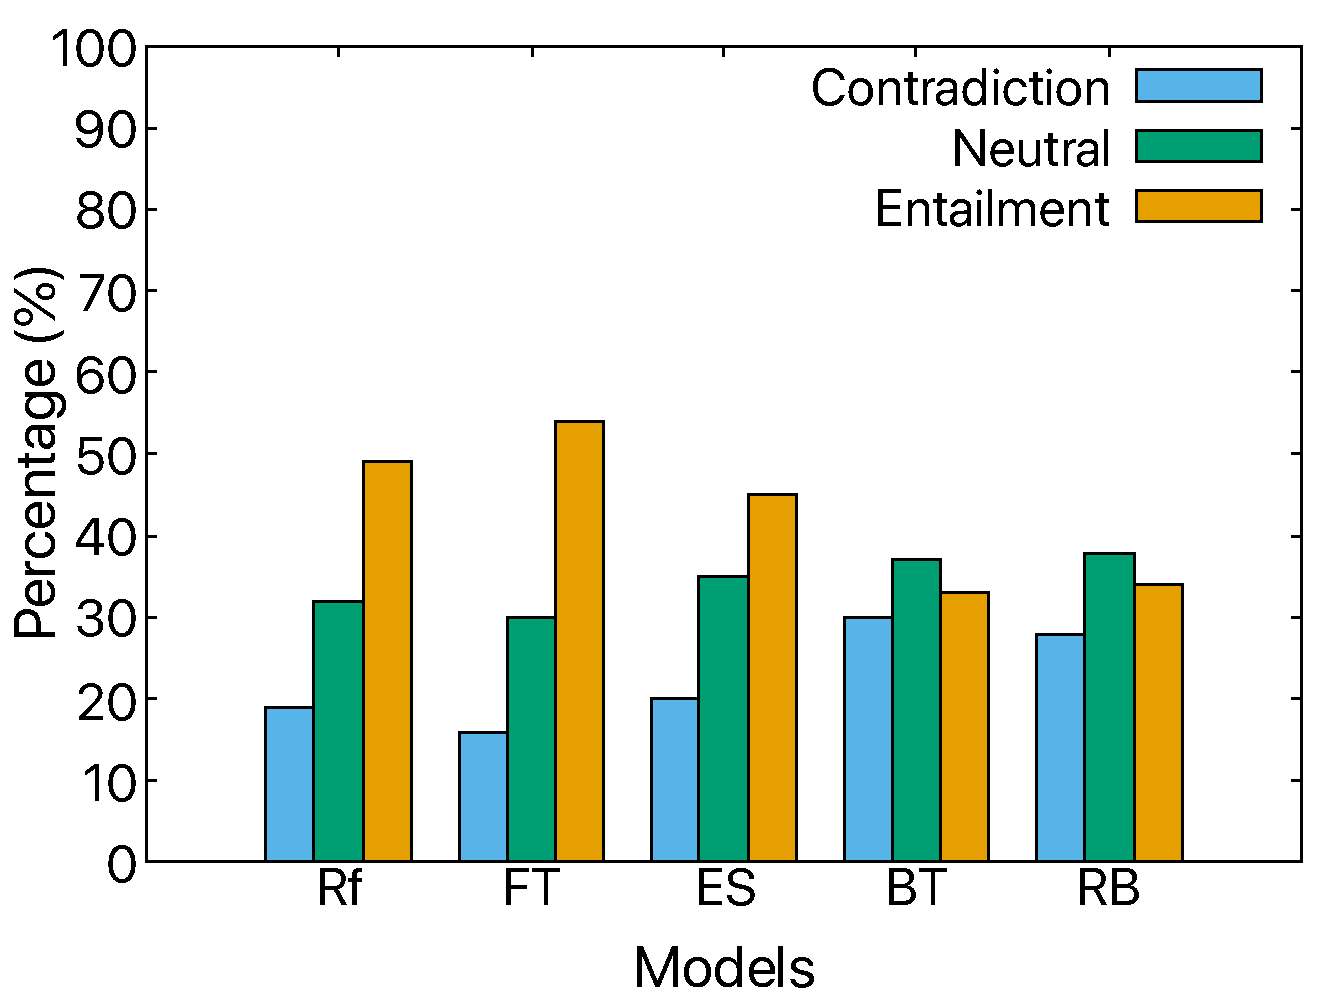
\includegraphics[width=\columnwidth]{picture/speaking-snli.pdf} 
\caption*{Cue ``speaking'' in SNLI}
\label{fig:cue_speaking}
\end{minipage}

\vspace{0.5cm}

\begin{minipage}[b]{0.45\linewidth}
\centering
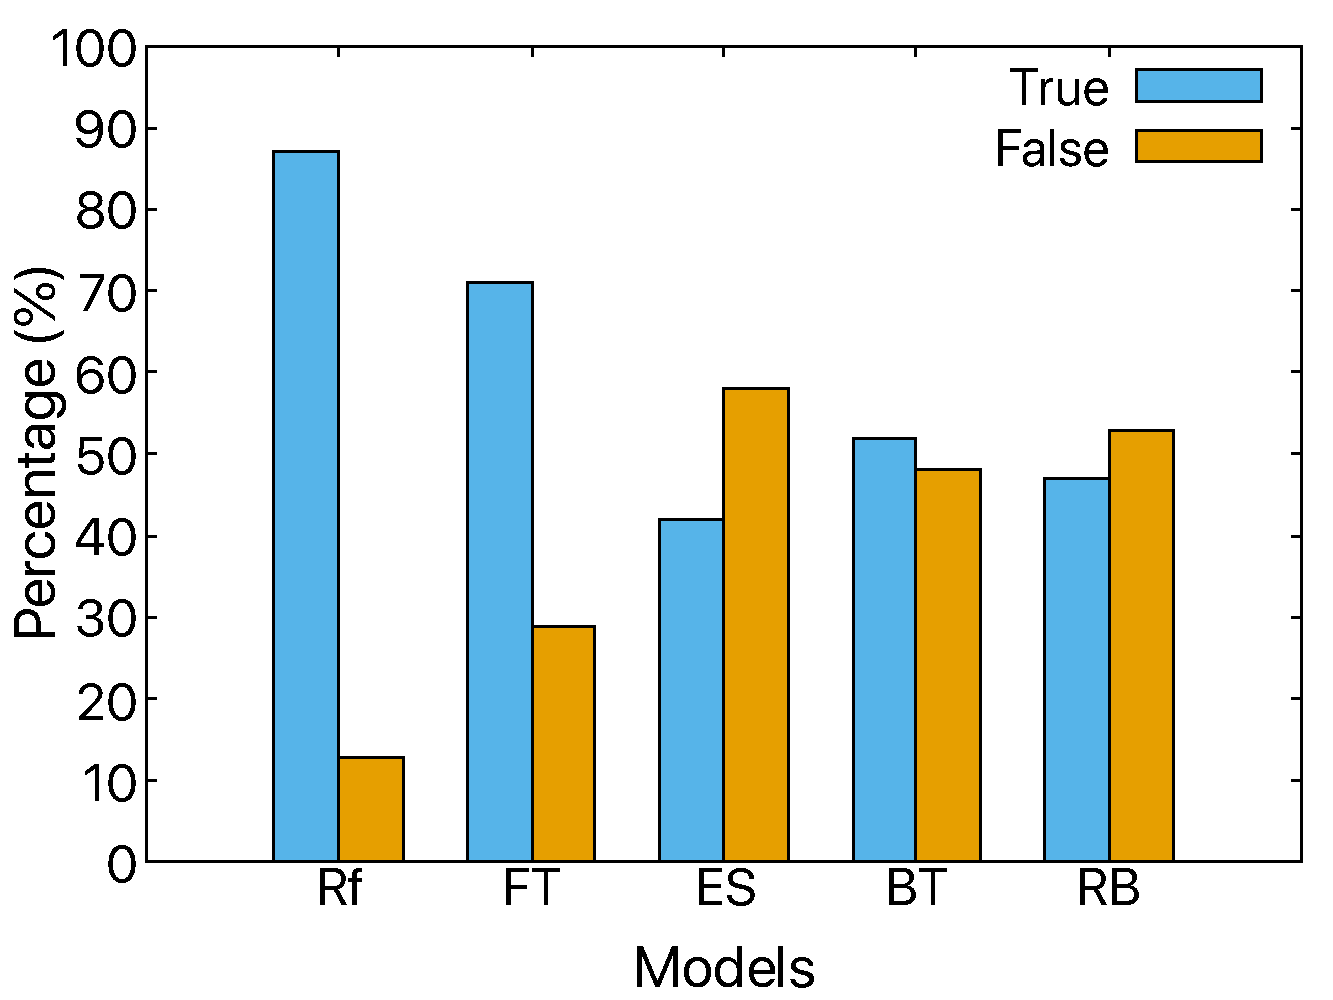
\includegraphics[width=\columnwidth]{picture/above-arct.pdf}
\caption*{Cue ``above'' in ARCT} 
\label{fig:cue_above} 
\end{minipage}
\hspace{0.5cm} 
\begin{minipage}[b]{0.45\linewidth} 
\centering 
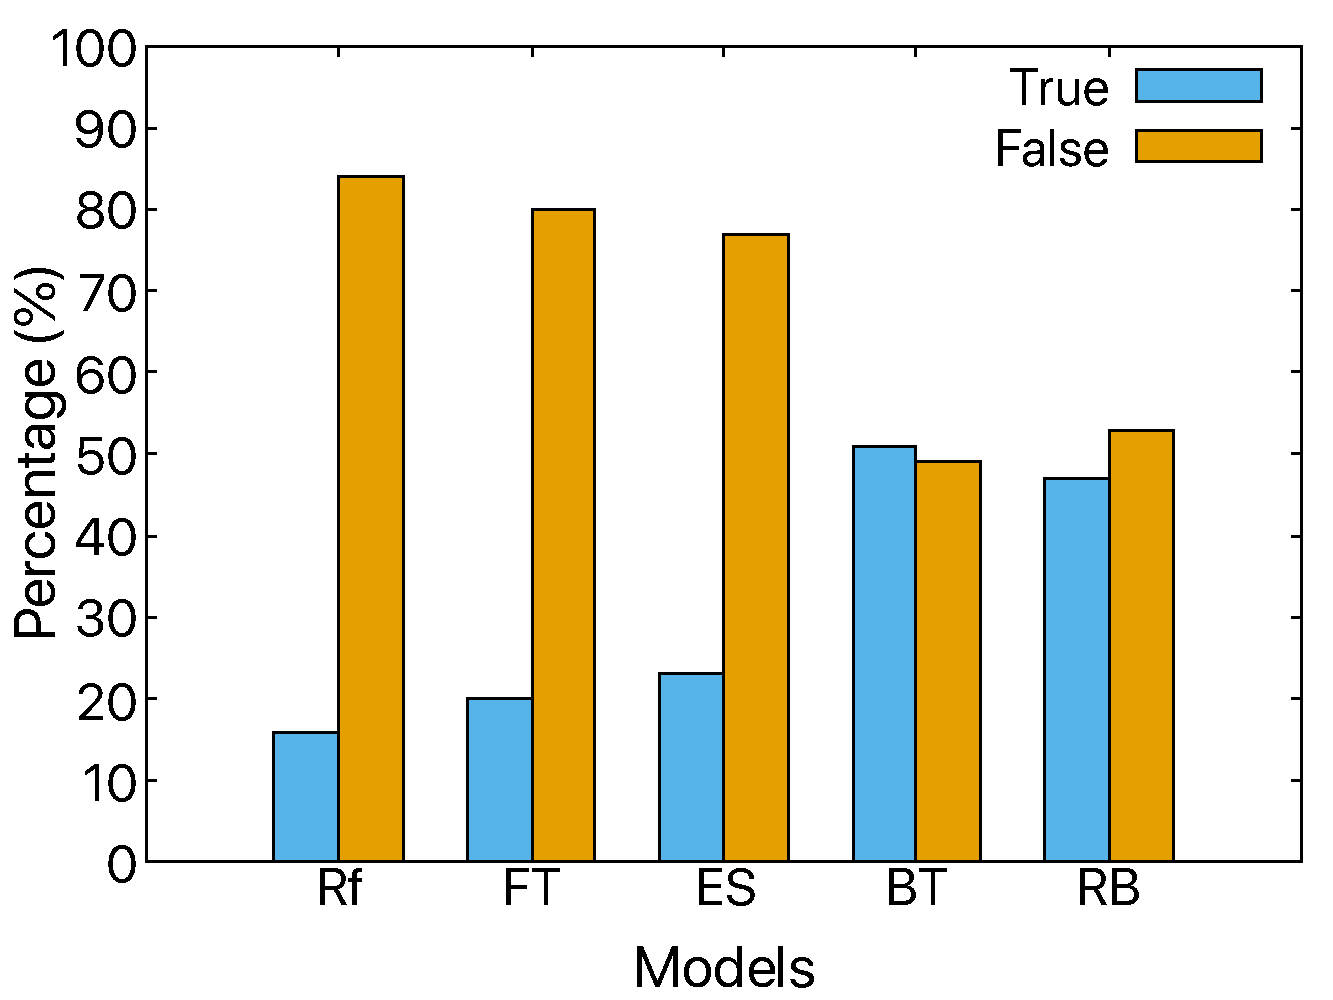
\includegraphics[width=\columnwidth]{picture/threw-roc.pdf} 
\caption*{Cue ``threw'' in ROC}
\label{fig:cue_threw}
\end{minipage}
\caption{Four test examples for distribution comparison with 4 different models}
\label{fig:cue_result}
\end{figure}

\textbf{Distribution Test:} We highlight three interesting findings in \figref{fig:cue_result}. The bars for the four models represent the distribution percentage based on each predicted label. $R_f$ denotes the extracted training data distribution with a specific feature. We observe that all models on the cue ``no'' in MNLI achieve positive $\Delta$ in \tabref{tab:bias}, particularly FastText. Consistent with the ``Accuracy Test,'' we find that the prediction label distribution skewness is amplified in \figref{fig:cue_result} for FastText and ESIM. With the ``no'' cue, they prefer to predict ``Contradiction'' even more than the ground truth in the training data. In contrast, BERT and RoBERTA moderately follow the training data. While the cue ``no'' is effective at influencing the models, the cue ``above'' is not as successful. \figref{fig:cue_result} shows that the distribution of predicted results for ESIM in ARCT is entirely opposite to the training data, explaining the $\Delta=-8.43$ in \tabref{tab:bias} and demonstrating that models may not exploit a cue even if it is present in the data. Similarly, ``speaking'' in BERT and RoBERTA can also explain their low $\Delta$ values, which are not shown in \tabref{tab:bias}.

The example of the cue ``threw'' presents an outlier for BERT, as the distribution test result is inconsistent with the accuracy test: the accuracy deviation is very high for BERT, but its prediction distribution is flat. We have not encountered many such contradictory cases. However, when they do occur, as in this example, we give BERT the benefit of the doubt that it might not have exploited the cue ``threw''. 



